\documentclass{article}
\usepackage{amsmath}
\usepackage{amssymb}
\usepackage{graphicx}
\usepackage{hyperref}
\usepackage[version=4]{mhchem}


\begin{document}
Hypotenuse \(A B\) of right \(\triangle A B C\) is divided into four congruent segments by points \(G, E\), and \(H\), in the order \(A, G, E, H\), and \(B\). If \(A B=20\), find the sum of the squares of the measures of the line segments from \(C\) to \(G, E\), and \(H\).\\
\centering
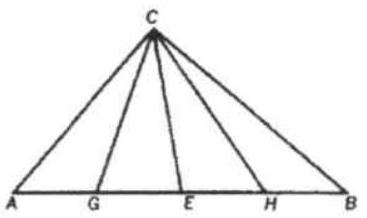
\includegraphics[width=\textwidth]{images/079(2).jpg}

Solution: 350 .\\
Draw \(C J\) perpendicular to \(A B\) at \(J\). Since \(A B=20, C E=10\).\\
Let \(G J=x\), and \(J E=5-x\).\\
By the Pythagorean Theorem, in right triangles \(\triangle C J G\) and \(\triangle C J E\),\\
\((C G)^{2}-x^{2}=10^{2}-(5-x)^{2}\)\\
\centering
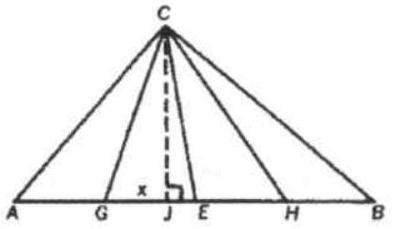
\includegraphics[width=\textwidth]{images/079(1).jpg}\\
or \((C G)^{2}=75+10 x\).\\
Similarly, in \(\triangle C J H\) and \(\triangle C J E,(C H)^{2}=(10-x)^{2}-(5-x)^{2}\), or \((C H)^{2}=175-10 x\).\\
By the addition of (1) and (2):\\
\((C G)^{2}+(C H)^{2}+(C E)^{2}=75+10 x+175-10 x+100=350\).


\end{document}
